\documentclass[dv_diss_main.tex]{subfiles}





%---------------------------------------------%
%----------------Figures----------------------
%---------------------------------------------%



\newcommand{\rddplot}{
\textit{Note.}This plot aggregate data into bins of half percentage points and estimate a third order polynomial regression between the running variable and the bins on each side of the cut-off. 
}


\newcommand{\rdd}{
\textit{Note.}This table reports the estimates of political alignment from equation (2). The sample includes post electoral years of all municipalities with close elections during the period 1998-2003. The outcome variables are measure as a three year changes. Controls refers to state fixed effects, election-year fixed effects, and baseline political characteristics (incumbency status, previous political alignment, previous political party). Mean dep var refers to the sample average of the outcome variable for the non-aligned municipalities. 
}



\newcommand{\sharerev}{
Percentage of revenues is the sample average share of each source of revenue on total revenues for the non-aligned counterparts
}

\newcommand{\shareemp}{
Percentage of employment is the sample average share of each sector on total employment for the non-aligned counterparts
}

\newcommand{\event}{
\textit{Note.}The figure plots the coefficients obtained from the estimation of equation (3) discussed in Section 4. The sample includes all municipalities with close elections during the period 1998-2003. The unit of observation is  the municipal-election pair, for each pair I follow the outcome measures in [-4 +4] years window. The outcome variables are measure in inverse hyperbolic sine points. The tick(thin) lines are 90\%(95\%) confidence intervals. The specification controls by municipality-election and election-year fixed effects. 
}

%inverse hyperbolic sine (IHS) transformation


\newcommand{\stars}{
Standard errors clustered at municipality level.  *** p<0.01, ** p<0.05, * p<0.1.
}

\newcommand{\census}{
}

\newcommand{\household}{
}

%example \newcommand{\rddnote}{\figtext{\justifying{\scriptsize{Notes:                }}}}
\newcommand{\starnotes}{* denotes significance at 10 pct., ** at 5 pct., and *** at 1 pct. level.}


%---------------------------------------------%
%----------------Figures----------------------
%---------------------------------------------%

%---External validity 

\newcommand{\sammi}{
\textit{Note.}This figure presents the difference of means of baseline covariates from the 2000 population census. Each point represents the estimate of the difference in means and the line the corresponding 95 percent confidence interval. All variables are standardized. Panel A shows the difference in means between the observational sample and the OLS-weighted sample. Panel B shows the difference in means between the observational sample and the IV-weighted sample. IV model weights are estimated using a control function approach. The weights are computed  based on Aronow and Samii (2016). We include as controls time and municipality fixed effects, formula's inputs and pre-trends of all outcomes of interest.
}

\newcommand{\sammidescrip}{
	
\textit{Note.}Means and standard deviations for baseline covariates from the 2000 population census. The column of the observational sample refers to the unweighted average. The OLS and IV columns correspond to weighted averages using regression-based weights of the corresponding models. The weights of the IV model are estimated using a control function approach. The weights are computed  based on Aronow and Samii (2016). We include as controls time and municipality fixed effect, formula's inputs and pre-trends of all outcomes of interest.

}

\newcommand{\revenuebydecil}{
\textit{Note.} Calculations based on information from SIMBAD (State and Municipal System Databases), National Institute of Statistics and Geography (INEGI).
}


\newcommand{\povertylineformula}{
\textit{Note.} The Figure shows the poverty line used to compute the formula on a yearly basis. We did not include the 2001 poverty line (Mex\$1097.859) for visualization purposes. Our estimation sample includes FAIS resources allocated between 2002-2014. 

}


\newcommand{\faisvariation}{\textit{Note.} The Figure plots the distribution of the share of transfer that corresponds to each state according to the FAIS formula. The figure plots the distribution of the demeaned shares across years by state  (2002-2014). Source: State FAIS formula values are collected from the Official Federal Gazette publication made on October of every year. }
\newcommand{\pcinequality}{
\textit{Note.} Calculations using the poverty maps of 2000, 2005, 2010, and 2014. Each quantile group is approximately 112 municipalities.
}

\newcommand{\pcincomegrowth}{
\textit{Note.} numbers reported are average across municipalities. The index shows the changes in a given percentile of the  municipal household income per capita distribution. Municipalities at the nth percentile in 2000 and 2014 do not necessarily correspond.
Source: Calculations using the poverty maps of 2000, 2005, 2010, and 2014.
}

\newcommand{\figurefaistrends}{
	
\textit{Note.}Panel A plots the share of municipalities reporting to receive zero resources from FAIS. Panel B plots the average value of per-capita transfers in constant prices, normalized to be 1 in 2005. Other public revenues include taxes, debt and unconditional cash transfers

}




%---------------------------------------------%
%----------------Tables----------------------
%---------------------------------------------%

\newcommand{\maintable}{\textit{Note.}Table entries correspond to separate regressions of an outcome,  listed on the leftmost column, on the independent variable specified in the column titles. Observations are the same across specifications that are in the same column. All monetary variables (intergovernmental transfers  and household per-capita income percentiles) are in logs, coverage and poverty headcount variables are in percentage points. Standard errors (in parentheses) are clustered at the municipality level to reflect the design effect and the autocorrelation of shocks over time. 2SLS estimates report the Kleibergen-Paap rk Wald F-statistic [in brackets]. 
}


\newcommand{\indicestables}{\textit{Note.}Table entries correspond to separate regressions of an outcome,  listed on the leftmost column, on the independent variable specified in the column titles. Observations are the same across specifications that are in the same column. All the outcomes indices that aggregate the information of all the variables that belong to a specific family. The infrastructure index aggregates the information of access to electricity, connection to sewerage, access to water,
quality of floor and access to sanitation. The poverty index aggregates the information of the inverse of log of per capita income and poverty rates measured by three poverty lines (food, capabilities and assets). The inequality index aggregates the information of Gini index and all income rations considered in the main results (90/10, 50/10 and 90/50). The index of each family is a linear combination of all the variables that belong to each family where the weights are based on \cite{anderson2008multiple}. Standard errors (in parentheses) are clustered at the municipality level. All  2SLS estimates report the Kleibergen-Paap rk Wald F-statistic [in brackets].
}


\newcommand{\firststage}{
\textit{Note.} The horizontal axis scale in logs but axis labels measure in constant pesos per capita of 2014. The plotted values correspond to mean-standardized residuals from transfers on a set of controls. Each color corresponds to a different specification: i) Purple, labeled as FE, includes municipality and time fixed effects. ii) light blue, labeled as FE+ Controls, includes the same set of fixed effects and two sets of time-varying controls: a) formula inputs, b) pre-policy trends outcome trends for all our outcomes of interest. 
}


\newcommand{\firststagetable}{
	\textit{Note.} This table presents estimates from regressing observed FAIS on law-implied FAIS transfers. Standard errors (in parenthesis) are clustered at the municipality level. Panel A adds sequentially the controls of our baseline specification across columns. The other panels add on top of that other set of time-varying controls. Panel B adds over the specifications of panel A the following sociodemographic controls: proportion of the adult population by education levels (primary, secondary and tertiary), the proportion of males and the dependency ratio. Panel C adds over the specifications of panel A the following economic controls: proportion of workers by sector (agriculture, manufacturing, construction, commerce, low-skill services and high skill services) and proportion of workers by type of occupation (abstract non-routine task, routine task, manual task, and non-routine manual tasks). 
	%Panel D adds over the specifications of panel A the following political controls: the size of public sector, the share of public workers with tertiary education, local revenue sources by type(own revenue, intergovernmental transfers both earmarked and non-earmarked). 
	In column (3) we use the assets poverty rate as a reference outcome to define the control used for pre-trends; results are robust to using any other outcome of interest as reference. \\
	\starnotes
}


\newcommand{\trendsdescrip}{
	\textit{Note.} Table entries in columns (1) and (2) correspond to separate regressions of an outcome, listed on the leftmost column, and our instrument in column titles. Outcome variables were measured as annual change between 1990 and 2000s. Coefficient estimates and robust standard errors (in parenthesis) correspond to cross-sectional regressions. Column (1) shows the unconditional correlation between the pre-policy trends and our instrument. Column (2) adds the formula's inputs as controls. Column (3) shows the mean and standard deviation of the pre-policy trends, measure as the average annual difference between 2000's and 1990 values. \\
	\starnotes
}




\newcommand{\mainresults}{
Column (1) reports OLS estimates of observed FAIS on outcomes of interest.
Column (2) reports reduce form estimates of law-implied FAIS.
Column (3) to (5) reports instrumental variable estimates of observed FAIS instrumented by law-implied FAIS. Column (3) includes standard controls, Column (4) has as additional control trends of the outcome of interest for the pre-policy period (1990-2000) interacted with year dummies. Column (5) includes time varying measures of all other source of municipal revenues: taxes, unconditional transfers and other conditional transfers. \\
\starnotes
}

\newcommand{\polynomial}{
	Column (1) reports our baseline specification for comparison purposes.
	Column (2) and Column (3) reports estimates from a specification that include as controls second and third order polynomials of the formula inputs. \\
	\starnotes
	
}

\newcommand{\trend}{
	Column (1) reports our baseline specification not accounting by pre-trends. 
	Column (2) corresponds to our baseline specification, it controls by pre-trend using the annual change in the outcome of interest between 1990-2000 interacted with a year dummy.
	Column (3) controls by pre-trends using the predicted level of the outcome of interest under linear trends assumption. 
	Column (4) controls by pre-trends using the lagged value of the outcome of interest. \\
	\starnotes
}

\newcommand{\urban}{
	Column (1) reports our baseline specification applied to the entire sample. 
	Column (2) reports our baseline specification for the subsample of municipalities with more than 15,000 inhabitants. Column (3) reports our baseline specification for the subsample of municipalities with less than 15,000 inhabitants. \\
	\starnotes
}





\newcommand{\mhtnote}{
		\textit{Note.} Table entries correspond to separate regressions of an outcome, listed on the leftmost column, on the variable specified in the column title. This table  present the estimates of our preferred specification, which corresponds to estimates of column 4 in Tables~\ref{tab:3},~\ref{tab:4} and~\ref{tab:5}. Standard errors (in parentheses) are clustered at the municipality level to reflect the design effect and the autocorrelation of shocks over time. Sharpened false discovery rate (FDR) q-values following Anderson (2008) in [brackets]. Family-wise p-values based on 2,000 bootstraps of the free step-down procedure of Westfall and Young (1993) in \{curly brackets\}. All monetary variables (intergovernmental transfers and household per-capita income percentiles) are in logs, coverage and poverty headcount variables are in percentage points. 
		\\
		\starnotes using conventional inference. 
}


\newcommand{\spendingcatalog}{
\textit{Note.}Each pair of Classification and sub-classification defines an authorized line  of spending authorized by FAIS spending catalog. Type abbreviations: Direct (D), Indirect (I), Complements (C.) and Specials (S)-most commonly used for natural disasters emergencies-. Modality abbreviations: C means construction, Eq means equipment, Ex means extension, I means installation, M means maintenance, R means rehabilitation, S means substitution, pre means preschool, pri means primary school, sec means secondary school and prep means high school. Source: Lineamientos Generales para la operación del FAIS (Anexo 1), February 14, 2014 https://ww.dof.gob.mx/nota_detalle.php?codigo=5332721&fecha=14/02/2014.
}


% Regressions include but do not report the lagged dependent variable, fixed effects for randomization blocks, and a set of LASSO-selected baseline covariates, and are weighted be representative of the eligible population. Standard errors (in parentheses) are clustered at the household level to reflect the design effect. Asterices denote significance at the 10, 5, and 1 percent levels, and are based on clustered standard errors, in parentheses. Anderson (2008) sharpened q-values presented in brackets. Variables marked with a † are in inverse hyperbolic sines. Reported p-values in final two columns derived from F-tests of hypotheses that cost-benefit ratios are equal between GD Main and Large transfer amounts (GD=GDL), and between Gikuriro and GD Large (GK=GDL).




\begin{document}

\begin{figure}[H]
\begin{center}
    \begin{tabular}[c]{ccc}
    
    \normalsize{\bf Panel A: Aggregate Spending} & & \normalsize{\bf Panel B: Shares by Categories} \\
    {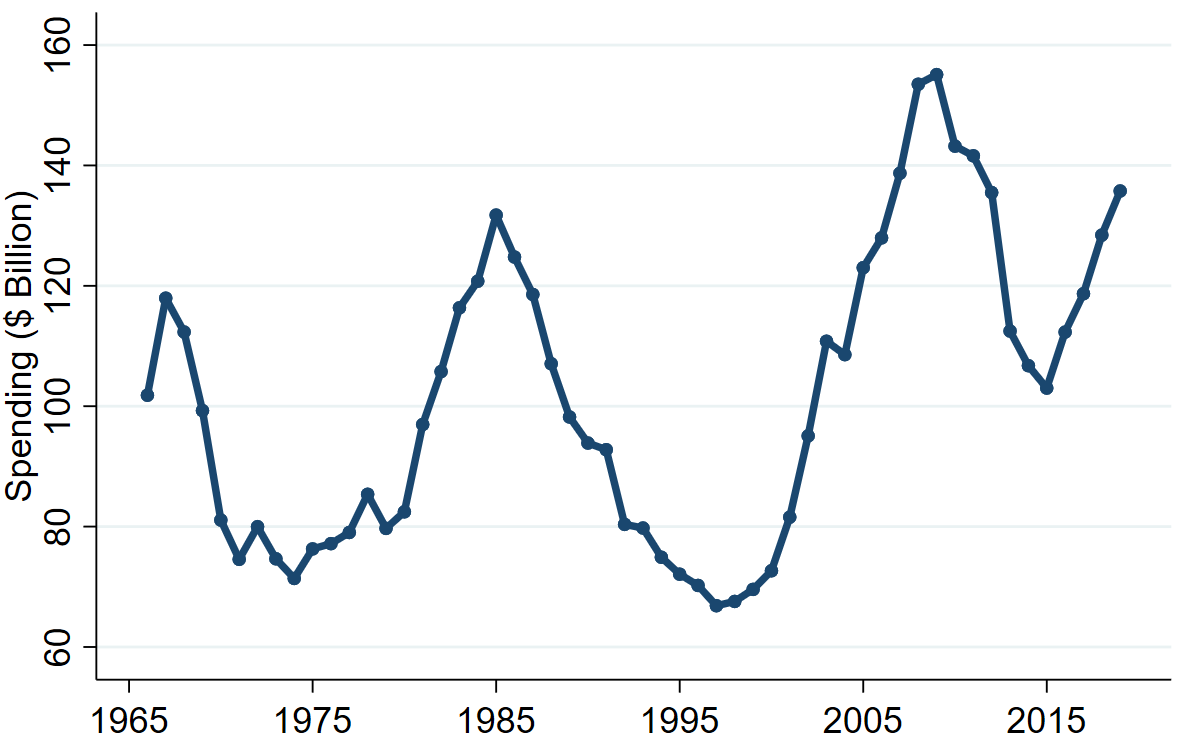
\includegraphics[height=1.8in,width=2.9in]{figures/graph_milspend_aggregate.png}} & & {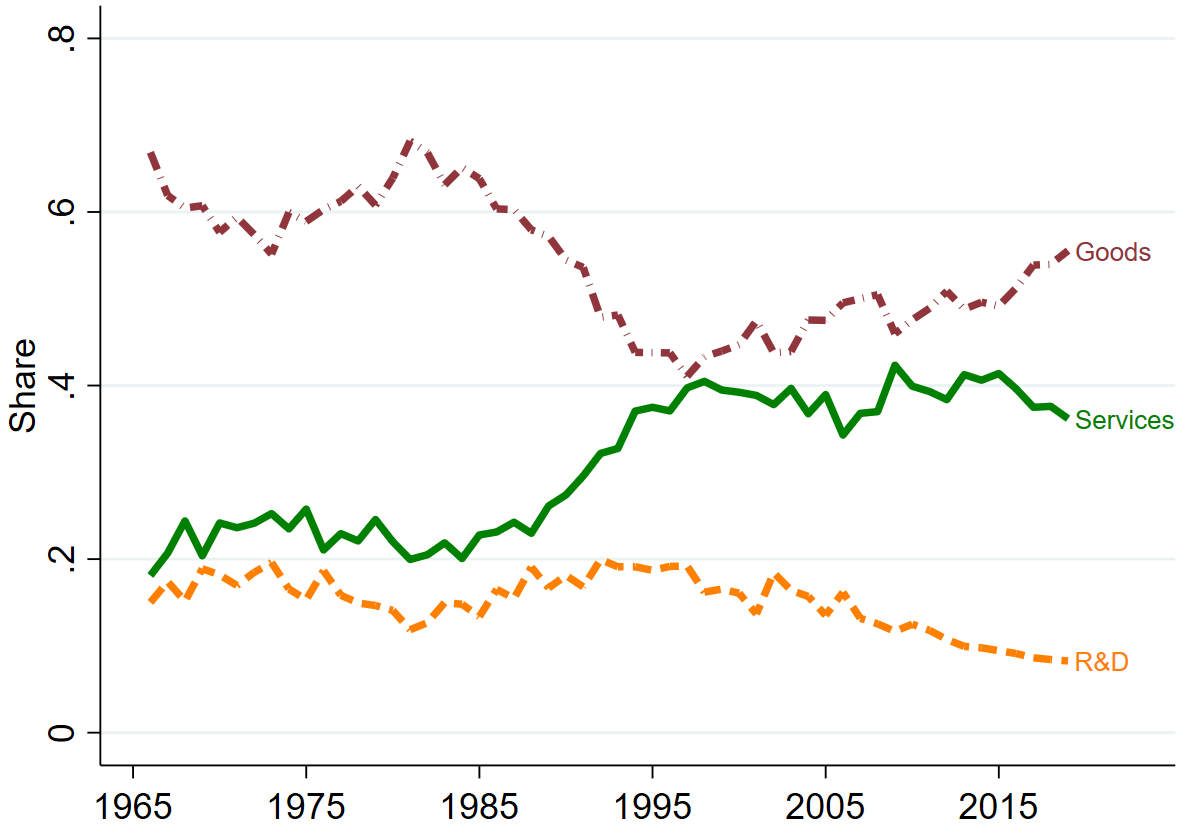
\includegraphics[height=1.8in,width=2.9in]{figures/graph_composition_shares.png}} \\[0.1in]
    
    \end{tabular}
   \caption{Military Spending}\label{fig:share_comp}
\end{center}
    
    
    \footnotesize{\textit{Note. } The national level statistics are calculated by aggregating the microdata on military procurement contracts available from NARA and USA Spending. Spending is in real terms by deflating the nominal value of a contract by the CPI. The classification of the spending into the three categories is based on the Federal supply classification code. The statistics are calculated by using more than $20$ millions of new contracts or modifications of existing contracts.}


\end{figure}
\newpage

\begin{figure}[H]
\begin{center}
    \begin{tabular}[c]{ccc}
    
    \normalsize{\bf Panel A: Total Spending} & & \normalsize{\bf Panel B: Spending in Goods} \\
    {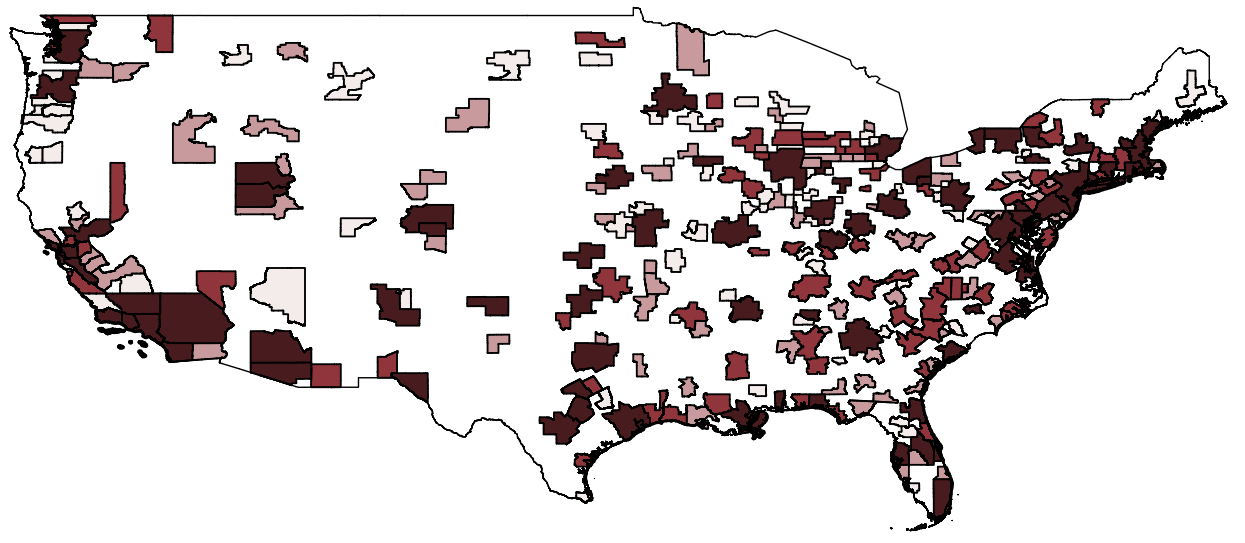
\includegraphics[height=1.5in,width=2.8in]{figures/map_cbsa_totspend.png}} & & {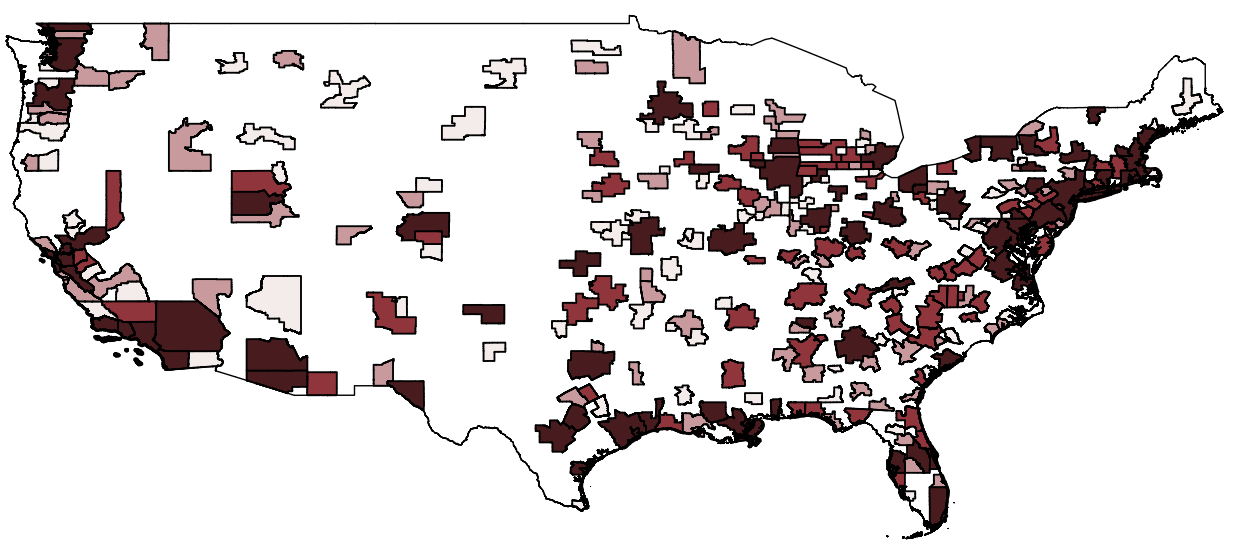
\includegraphics[height=1.5in,width=2.8in]{figures/map_cbsa_goodsspend.png}} \\[0.1in]
    
    \normalsize{\bf Panel C: Spending in Services} & & \normalsize{\bf Panel D: Spending in R\&D} \\
    {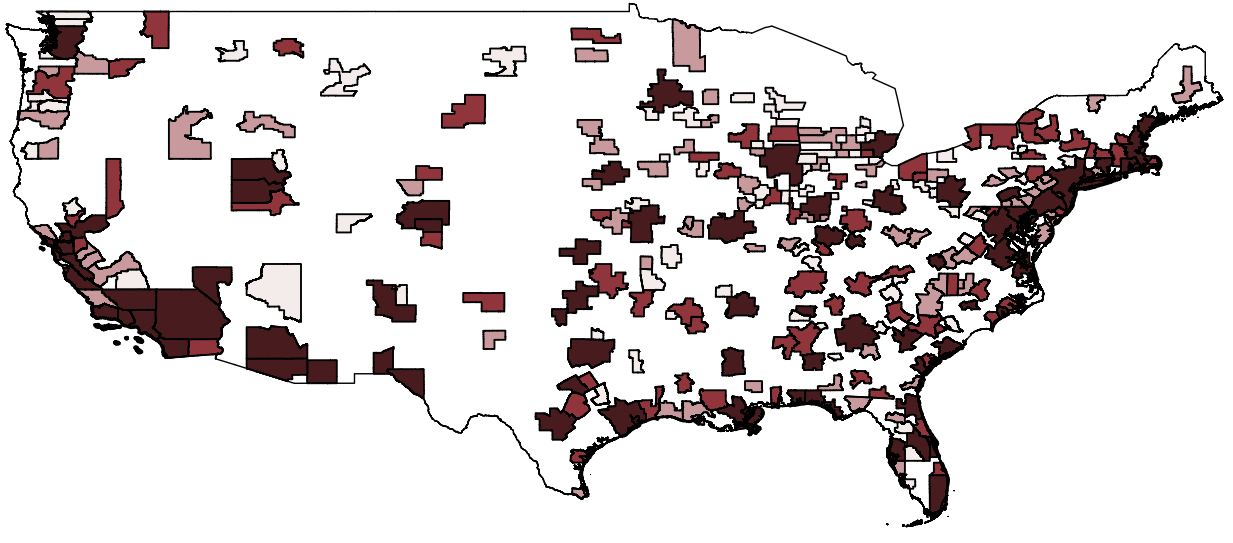
\includegraphics[height=1.5in,width=2.8in]{figures/map_cbsa_servicesspend.png}} & & {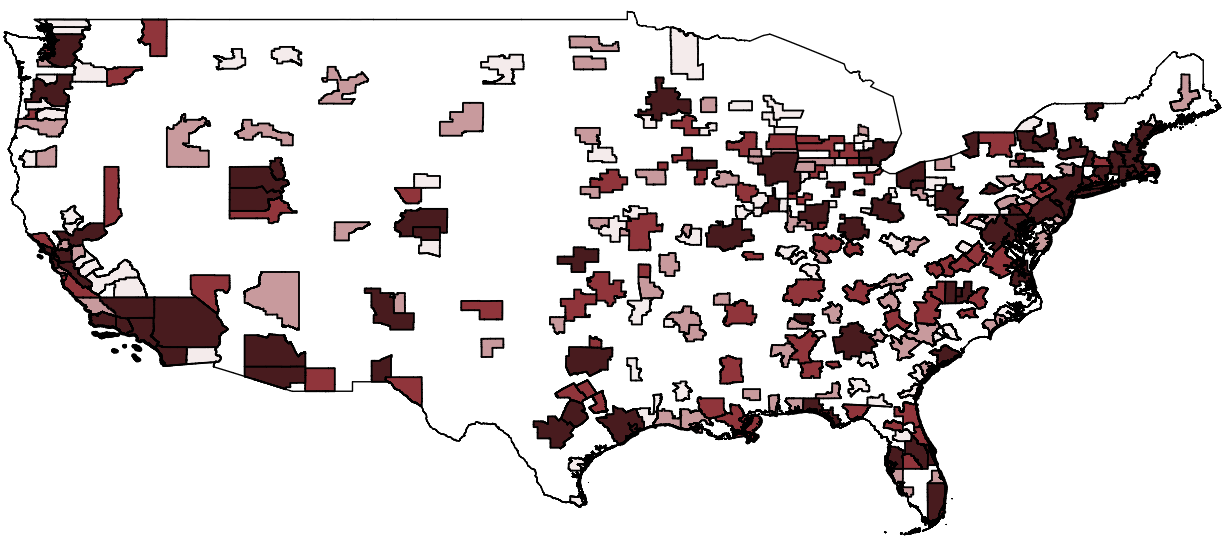
\includegraphics[height=1.5in,width=2.8in]{figures/map_cbsa_rdspend.png}} \\[0.1in]
    
    \multicolumn{3}{c}{
\includegraphics[height=0.2in,width=3.8in]{figures/map_cbsa_legspend.png}} \\[0.1in]
      \end{tabular}
     \caption{Military Spending - Geographic Distribution}
\end{center}
   
    \footnotesize{\textit{Note. } The quartile to which a MSA belongs is assigned based on the average military spending in real terms that the MSA receives over the period $1966-2019$. The classification of the spending into the three categories is based on the Federal supply classification code. The maps only show the $296$ MSAs included in our sample.}
    \label{fig:map_spend}
\end{figure}
\newpage

\begin{figure}[H]
    \begin{center}
    \begin{tabular}[c]{ccc}
    
    \normalsize{\bf Panel A: Total Spending} & & \normalsize{\bf Panel B: Spending in Goods} \\
    {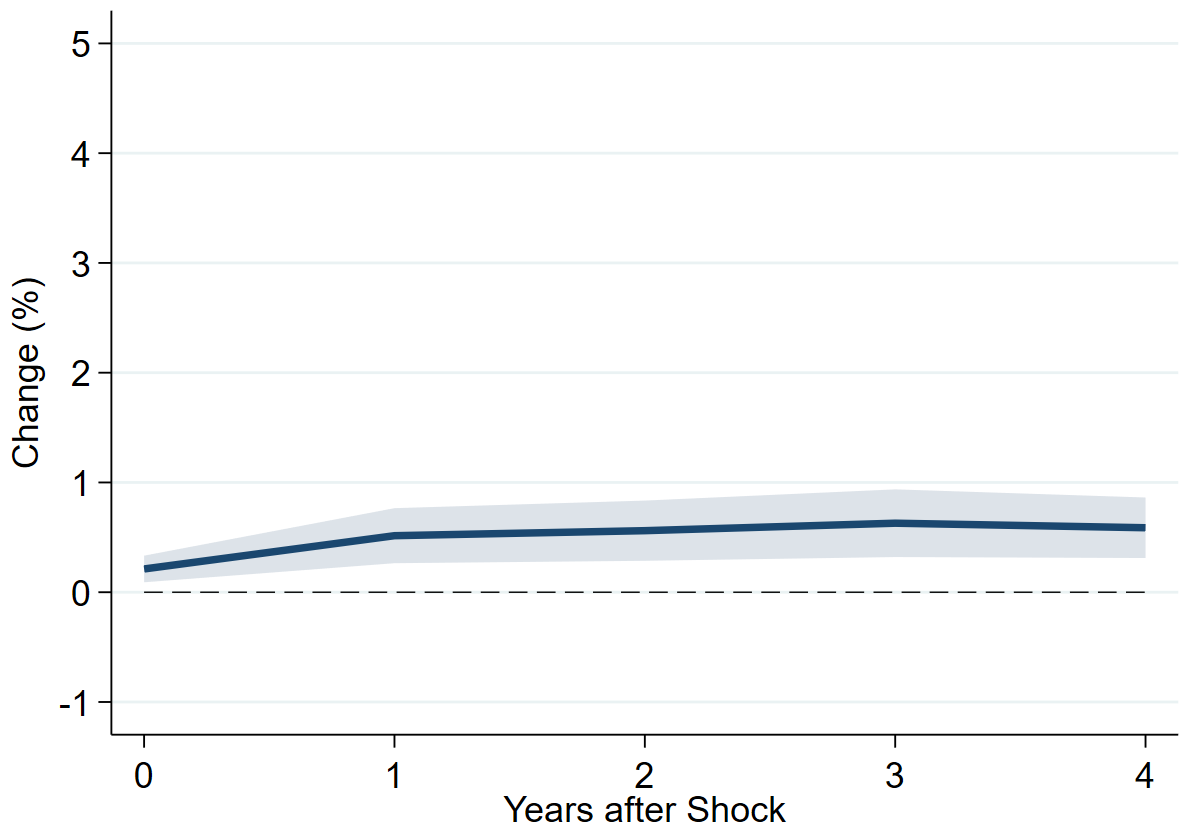
\includegraphics[height=1.5in,width=2.8in]{figures/graph_Rn_wages_lv_Rn_ms_lv.png}} & & {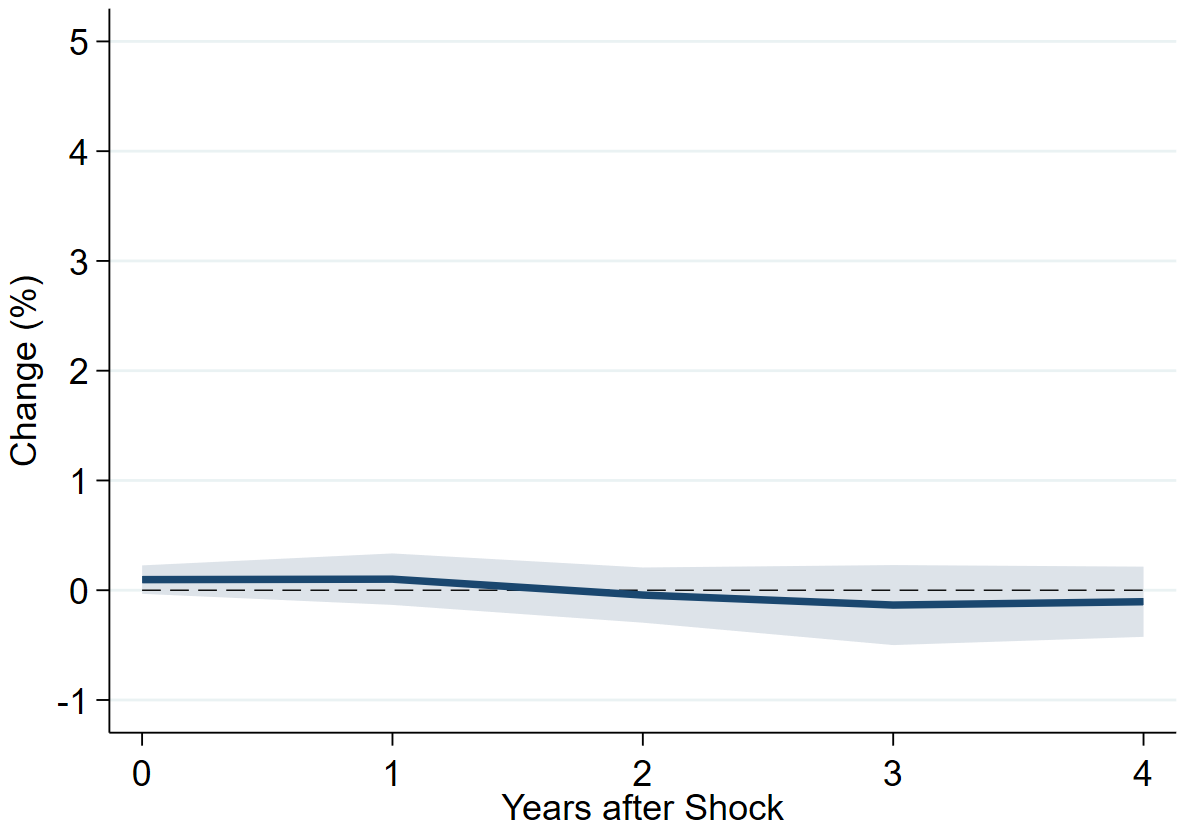
\includegraphics[height=1.5in,width=2.8in]{figures/graph_Rn_wages_lv_Rn_ms_goods_lv.png}} \\[0.1in]
    
    \normalsize{\bf Panel C: Spending in Services} & & \normalsize{\bf Panel D: Spending in R\&D} \\
    {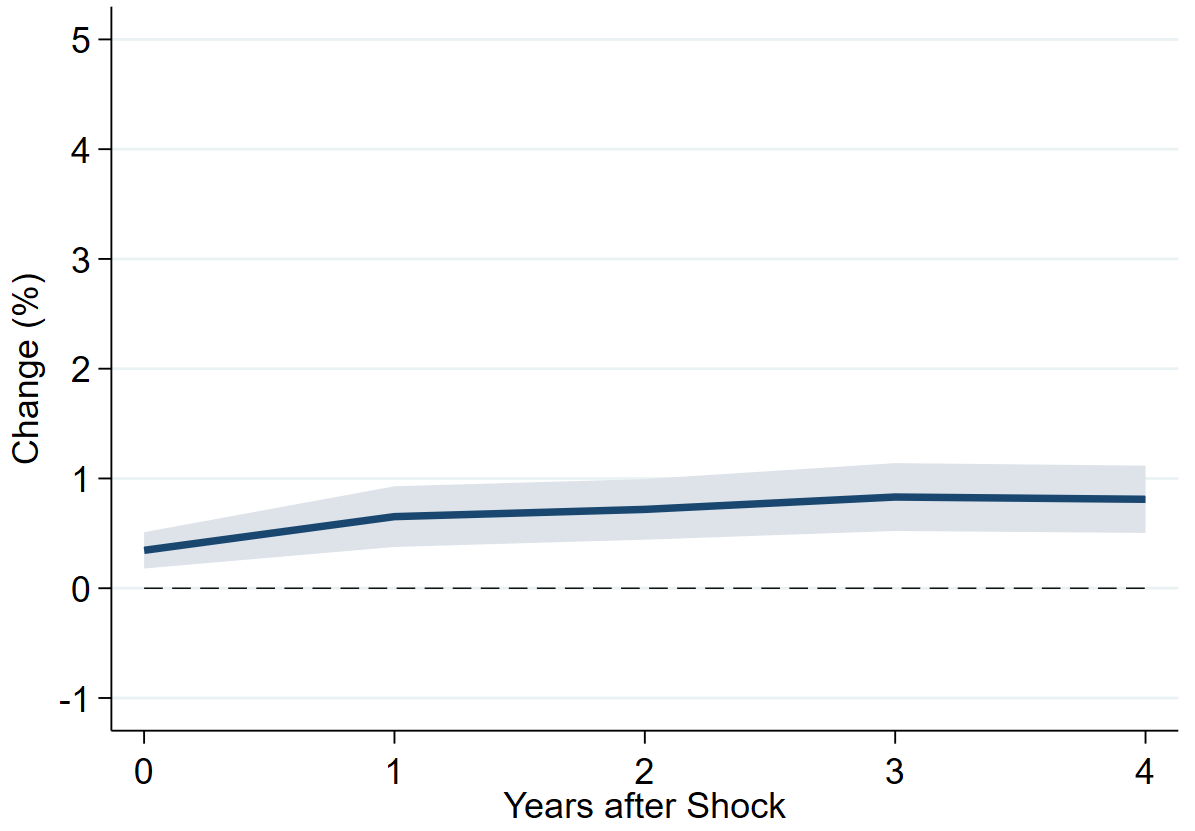
\includegraphics[height=1.5in,width=2.8in]{figures/graph_Rn_wages_lv_Rn_ms_services_lv.png}} & & {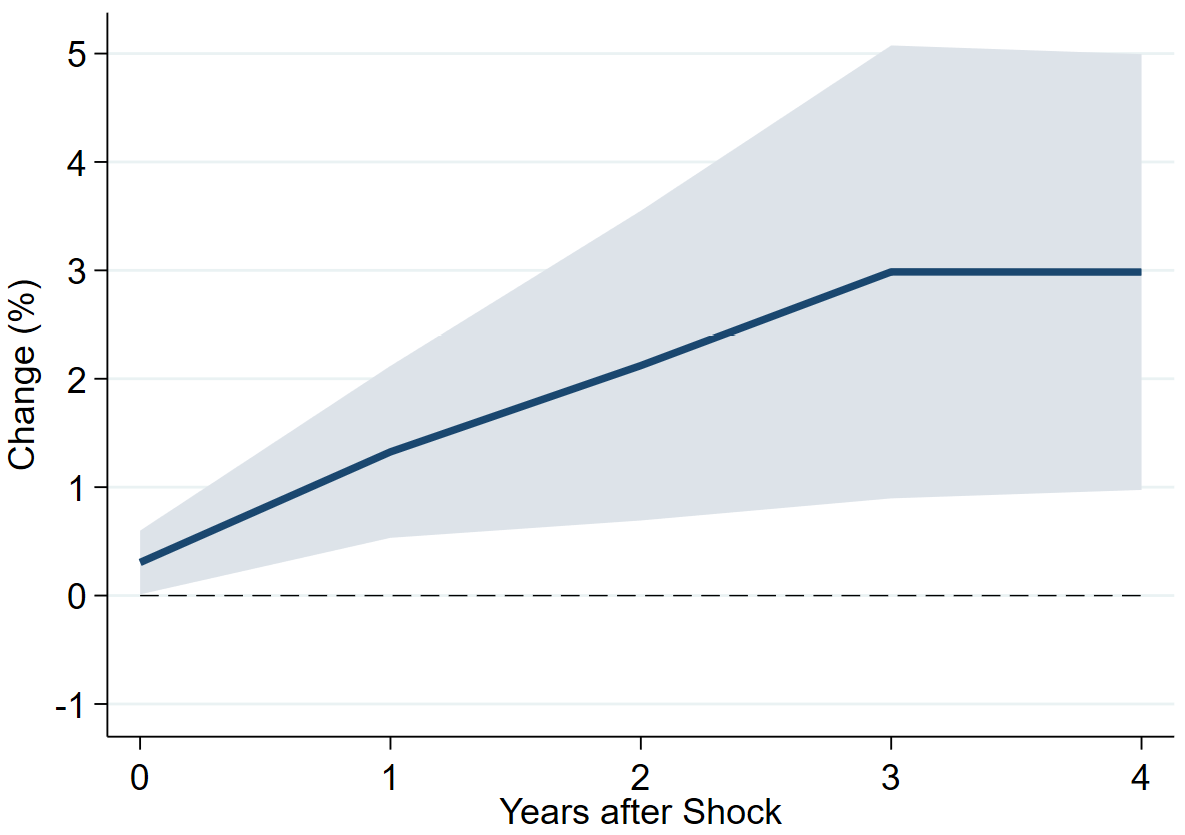
\includegraphics[height=1.5in,width=2.8in]{figures/graph_Rn_wages_lv_Rn_ms_rd_lv.png}} \\[0.1in]
    
    
    
    \end{tabular}
        \caption{Fiscal Multipliers - Earnings}
    \end{center}
    

 
    \footnotesize{\textit{Note. } Panel A reports the estimates from equation \eqref{eq:fm_base}. The remaining panels the estimates from equation \eqref{eq:fm_comp}. We use the instrumental variable approach with the instrument calculated as in equation \eqref{eq:fm_iv}. The unit of observations are MSAs in different years. The balanced panel used for computing the estimates includes $296$ MSAs for the period $1980-2015$. The instrument is calculated using observations between $1966$ and $1980$. Standard errors are clustered at MSA-level. The shaded areas report the $90\%$ confidence intervals.}

    \label{fig:fm_earnings}
\end{figure}
\newpage

\begin{figure}[H]
    \begin{center}
    \begin{tabular}[c]{ccc}
    
    \normalsize{\bf Panel A: Total Spending} & & \normalsize{\bf Panel B: Spending in Goods} \\
    {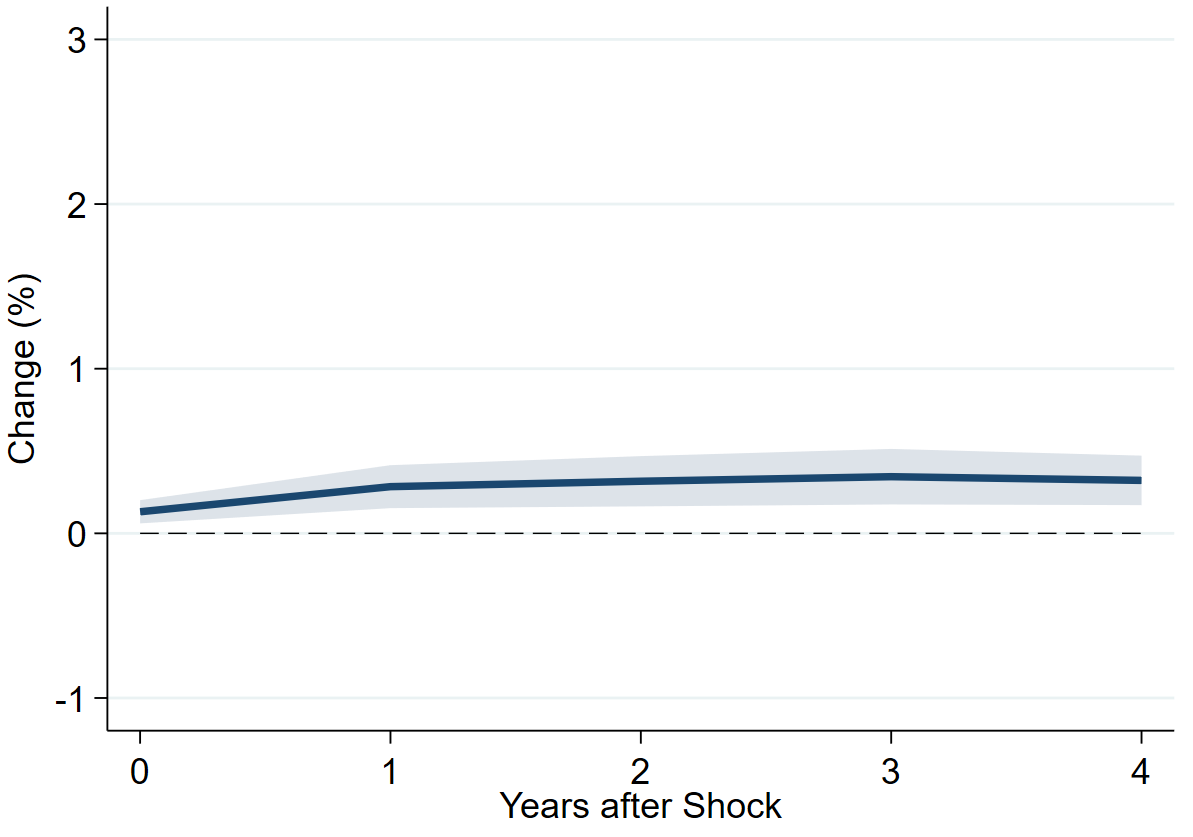
\includegraphics[height=1.5in,width=2.8in]{figures/graph_Rn_emp_lv_Rn_ms_lv.png}} & & {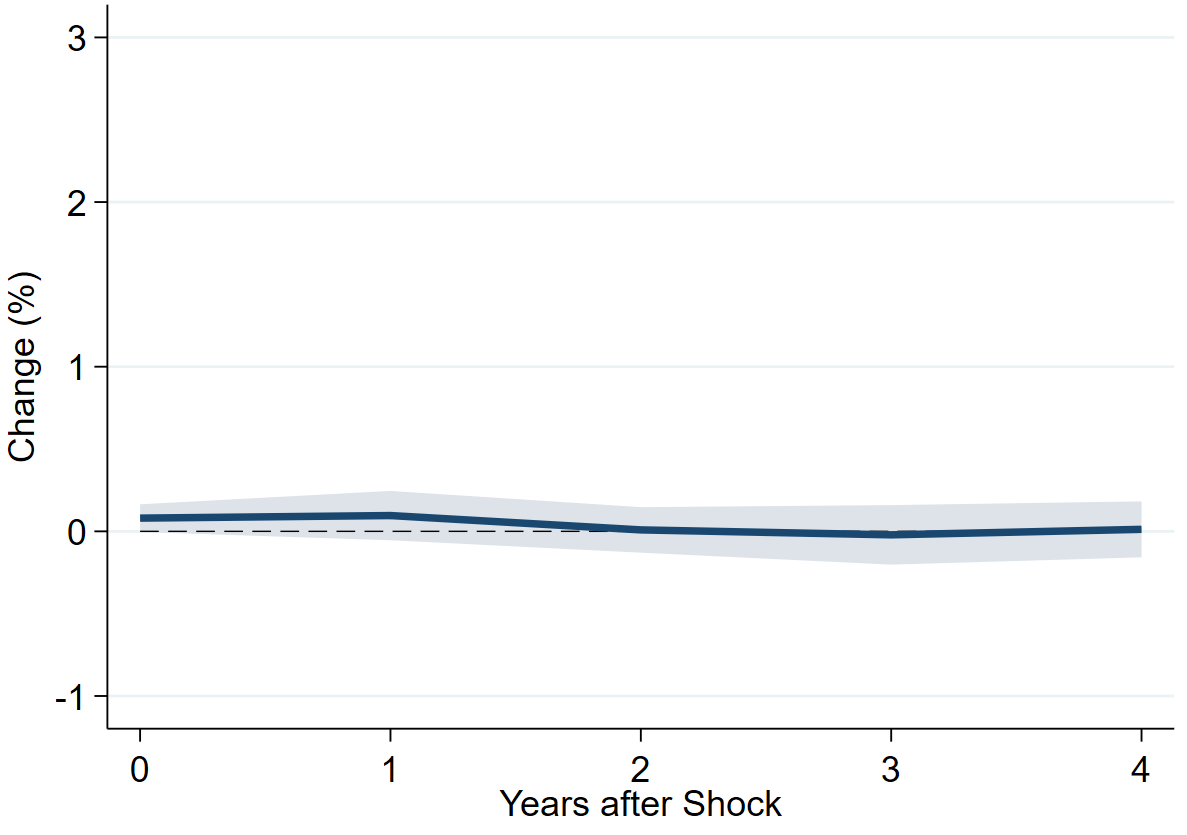
\includegraphics[height=1.5in,width=2.8in]{figures/graph_Rn_emp_lv_Rn_ms_goods_lv.png}} \\[0.1in]
    
    \normalsize{\bf Panel C: Spending in Services} & & \normalsize{\bf Panel D: Spending in R\&D} \\
    {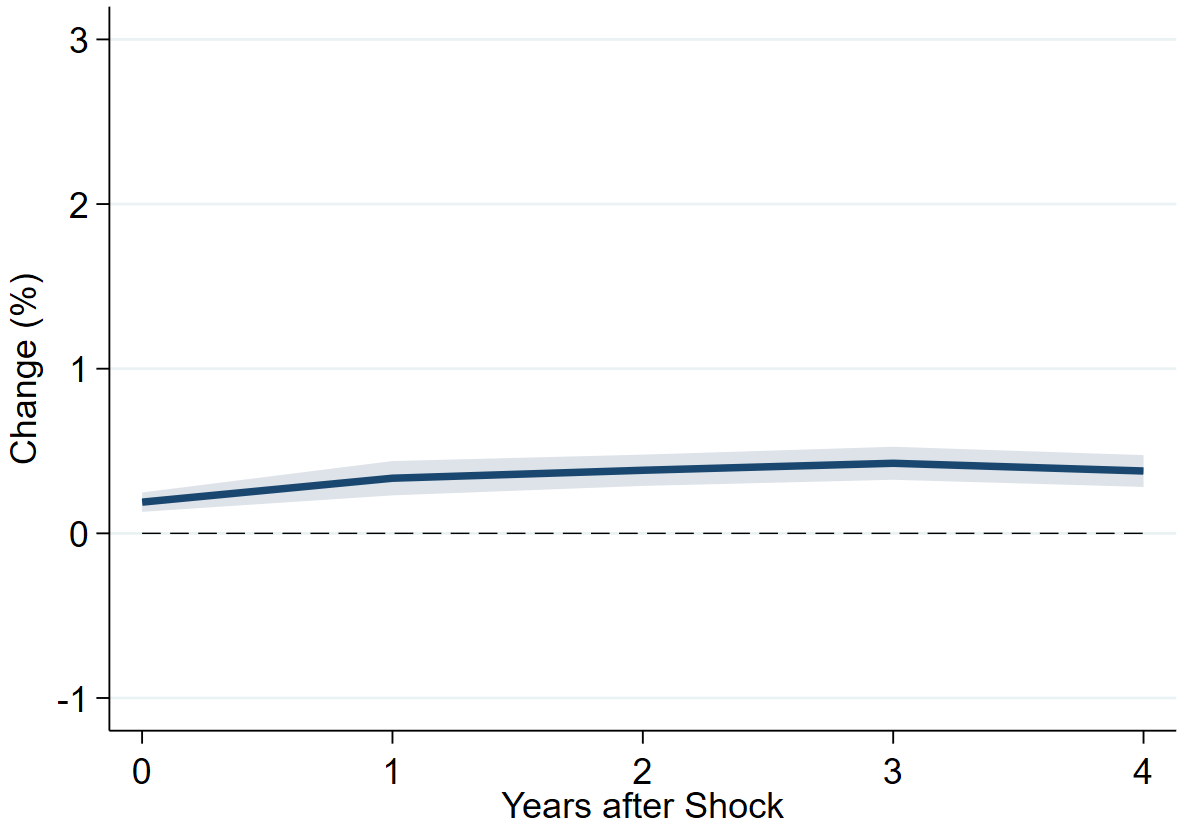
\includegraphics[height=1.5in,width=2.8in]{figures/graph_Rn_emp_lv_Rn_ms_services_lv.png}} & & {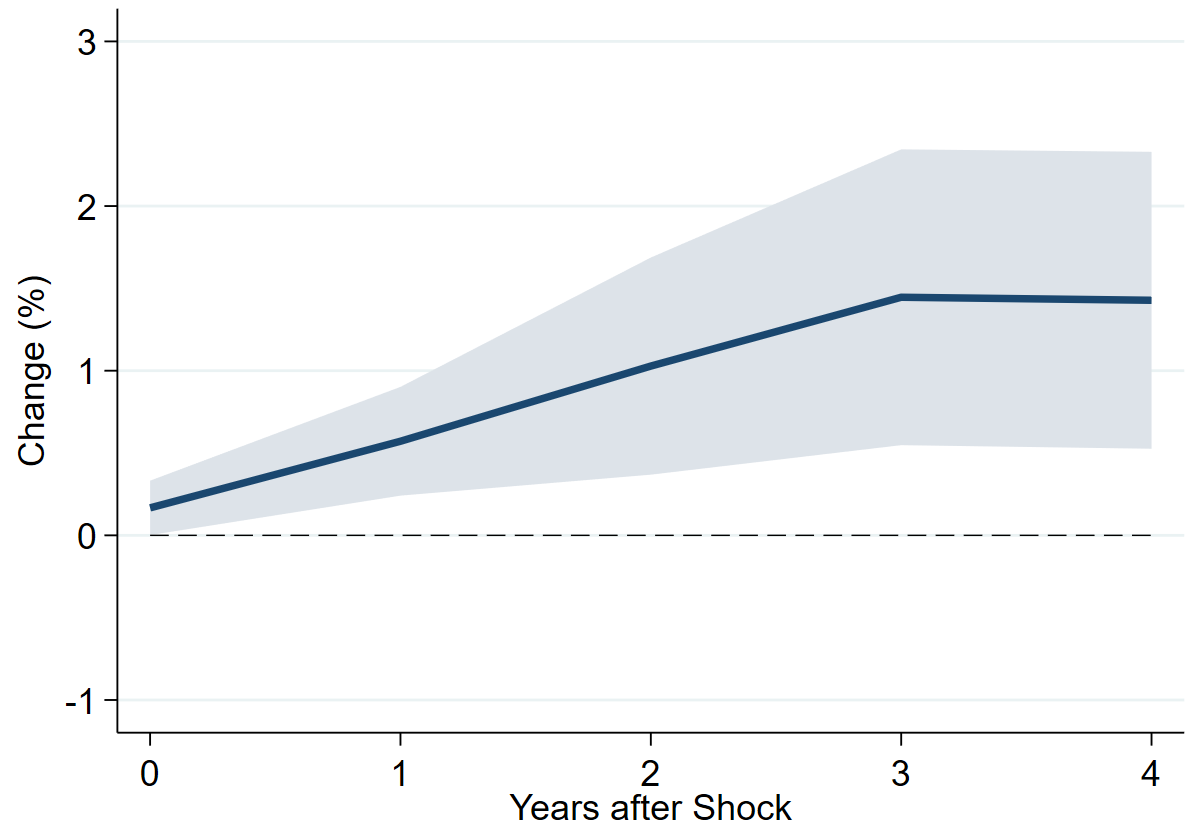
\includegraphics[height=1.5in,width=2.8in]{figures/graph_Rn_emp_lv_Rn_ms_rd_lv.png}} \\[0.1in]
    
    \end{tabular}
    \caption{Fiscal Multipliers - Employment}
    \end{center}
    
    \footnotesize{\textit{Note. } Panel A reports the estimates from equation \eqref{eq:fm_base}. The remaining panels the estimates from equation \eqref{eq:fm_comp}. We use the instrumental variable approach with the instrument calculated as in equation \eqref{eq:fm_iv}. The unit of observations are MSAs in different years. The balanced panel used for computing the estimates includes $296$ MSAs for the period $1980-2015$. The instrument is calculated using observations between $1966$ and $1980$. Standard errors are clustered at MSA-level. The shaded areas report the $90\%$ confidence intervals.}
    \label{fig:fm_employment}
\end{figure}
\newpage

\begin{figure}[H]
    \begin{center}
        \begin{tabular}[c]{c}
   
    {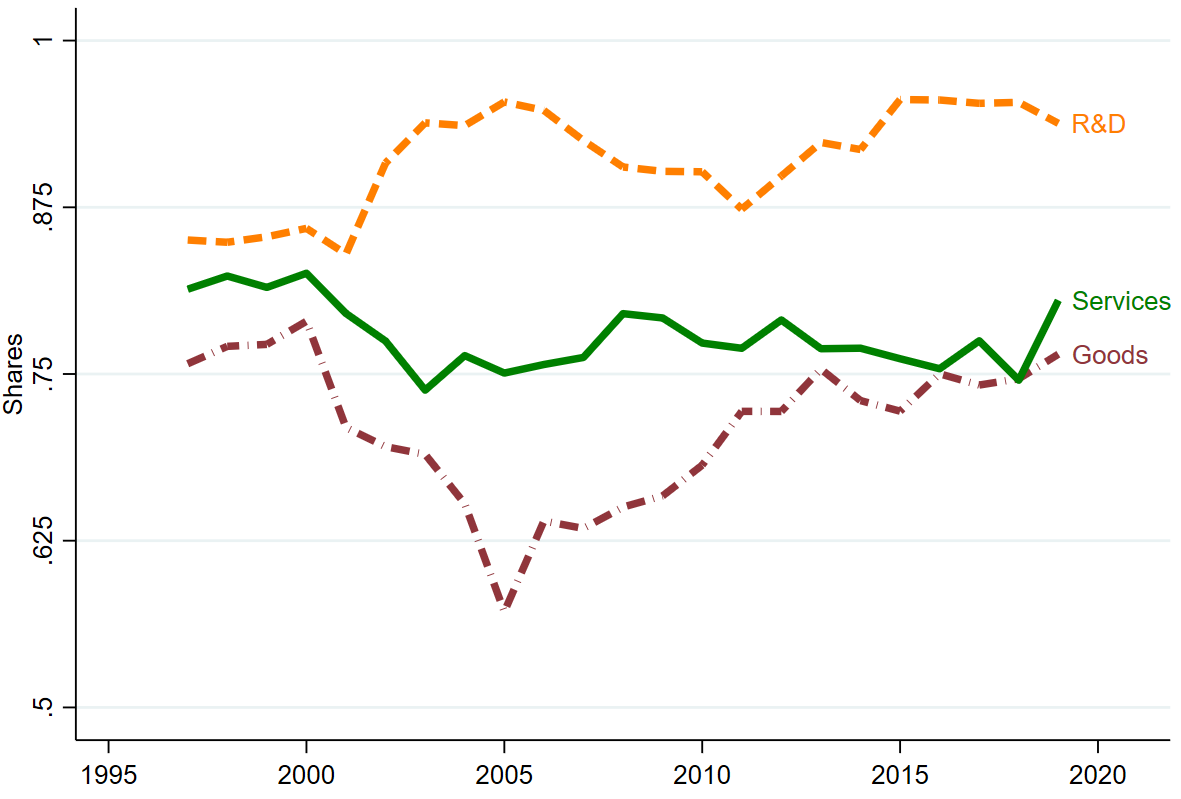
\includegraphics[height=2.5in,width=4.5in]{figures/graph_share_laborintensity.png}} \\[0.1in]

    
    \end{tabular}
    \caption{Share of Spending in Labor-intensive Industries}
    \end{center}
    
    
    \footnotesize{\textit{Note. } The classification of the spending into the three categories is based on the Federal supply classification code. The classification between low and high labor-intensive industries is based on the value added data collected from the BEA.}
    \label{fig:shlabint_comp}
\end{figure}
\newpage

\begin{figure}[ht]
    \begin{center}
    \begin{tabular}[c]{ccc}
    
    \normalsize{\bf Panel A: Total Spending} & & \normalsize{\bf Panel B: Spending in Goods} \\
    {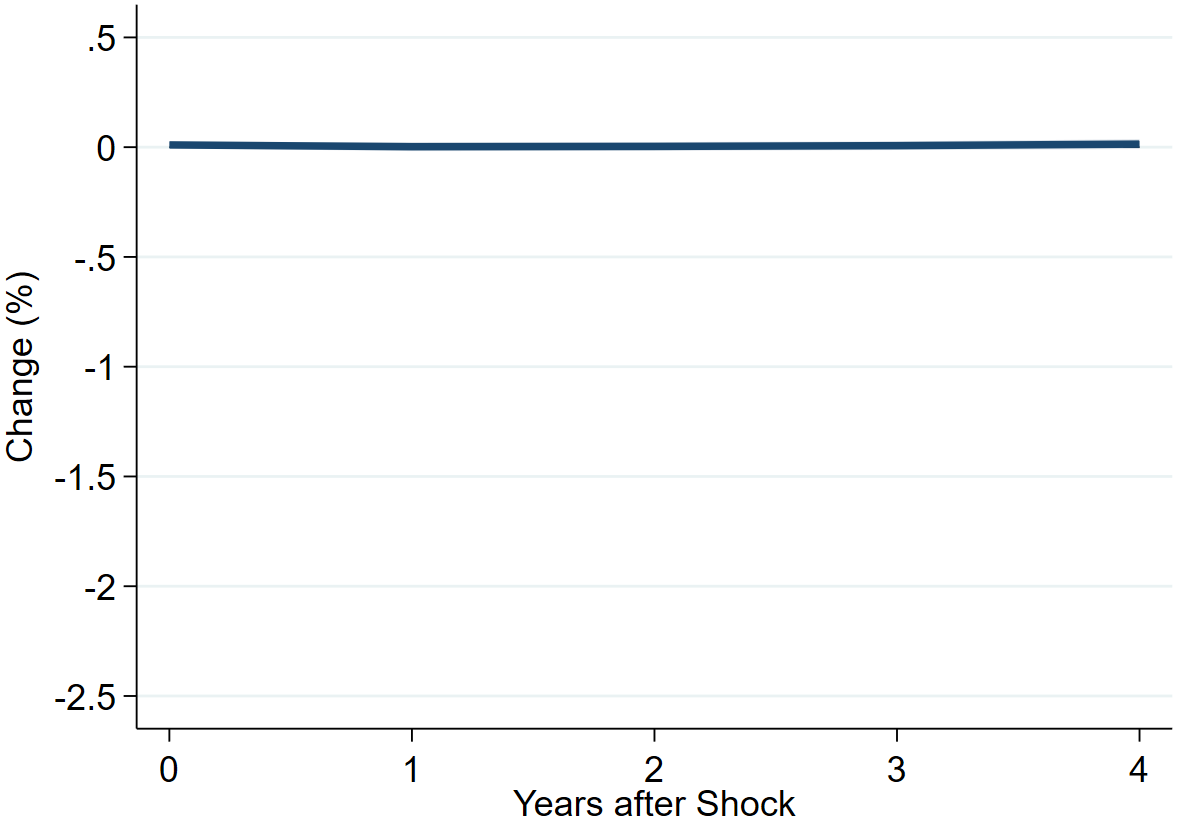
\includegraphics[height=1.5in,width=2.8in]{figures/graph_Rn_wages_lv_spill100_Rn_ms_lv_spill100.png}} & & {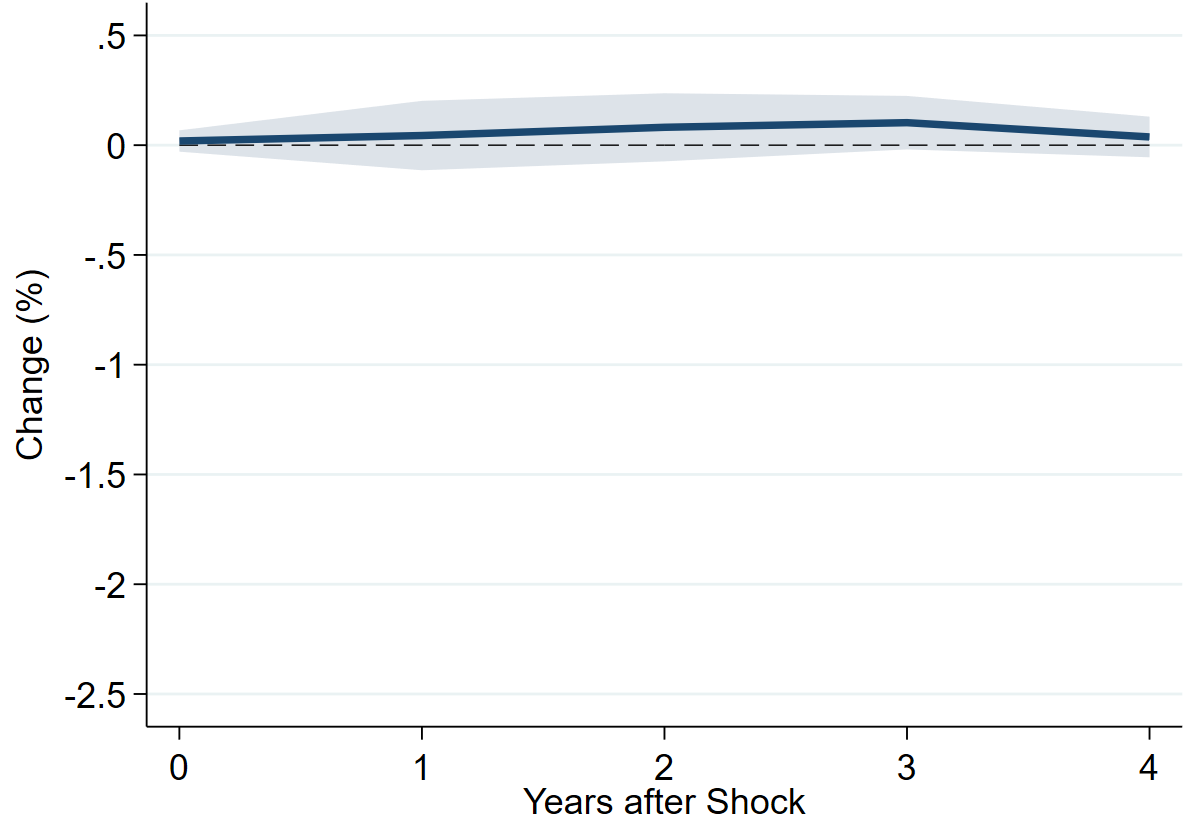
\includegraphics[height=1.5in,width=2.8in]{figures/graph_Rn_wages_lv_spill100_Rn_ms_goods_lv_spill100.png}} \\[0.1in]
    
    \normalsize{\bf Panel C: Spending in Services} & & \normalsize{\bf Panel D: Spending in R\&D} \\
    {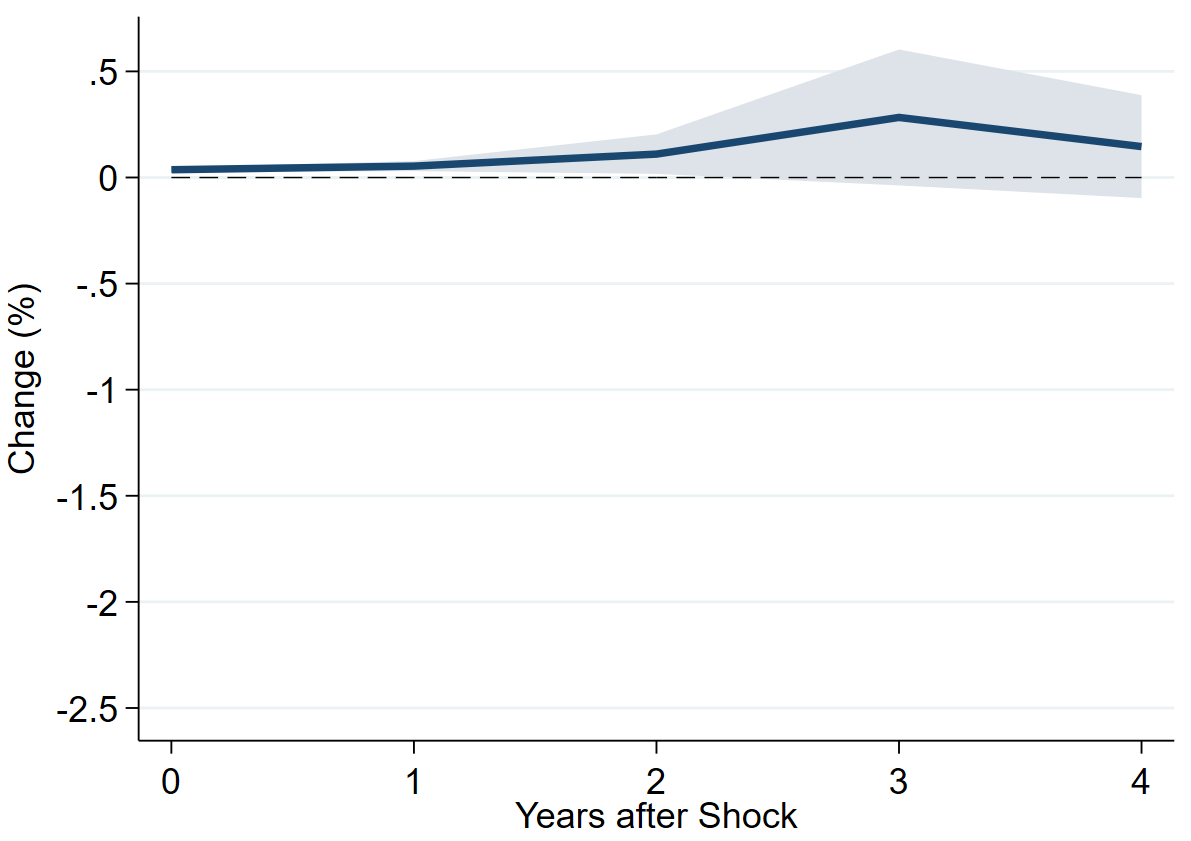
\includegraphics[height=1.5in,width=2.8in]{figures/graph_Rn_wages_lv_spill100_Rn_ms_services_lv_spill100.png}} & & {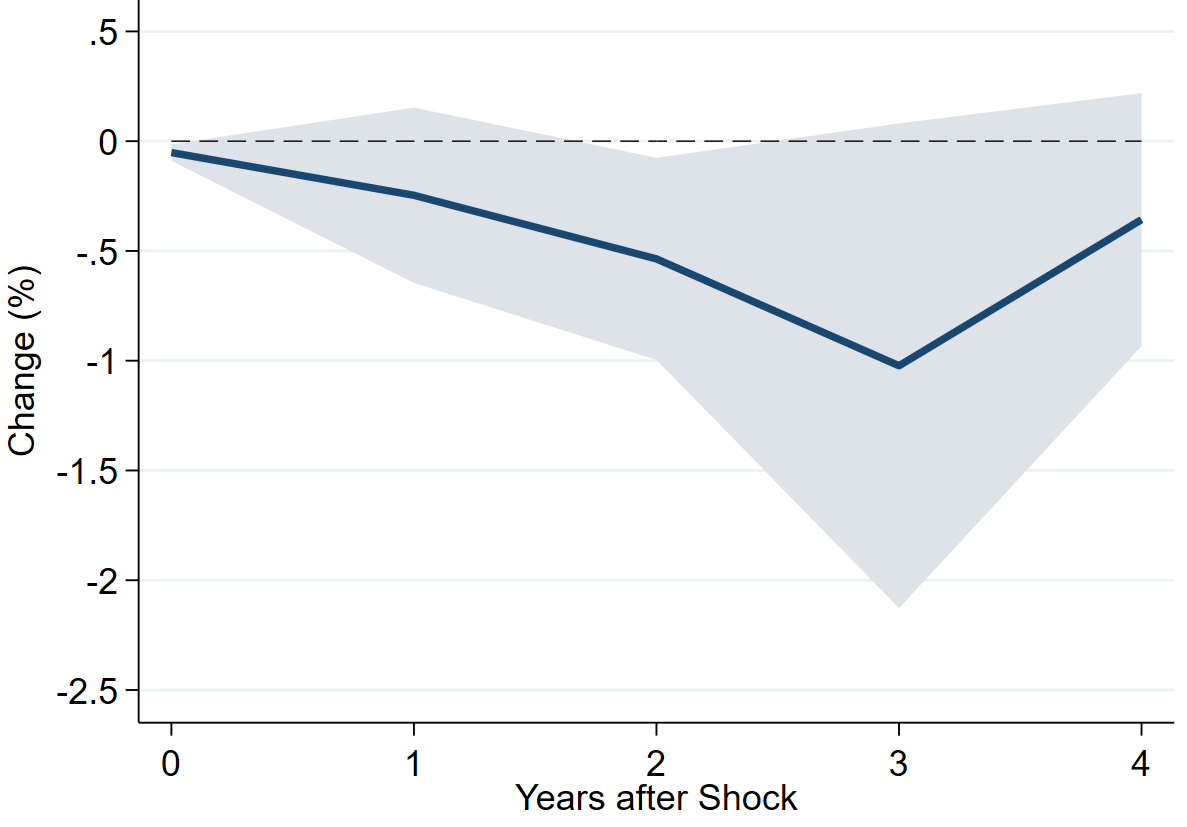
\includegraphics[height=1.5in,width=2.8in]{figures/graph_Rn_wages_lv_spill100_Rn_ms_rd_lv_spill100.png}} \\[0.1in]
    
    \end{tabular}
    \caption{``Outflow'' Effects - Earnings}
    \end{center}
    
    
    
    \footnotesize{\textit{Note. } Estimates are computed from  equation \eqref{eq:fm_spill}. We use the instrumental variable approach with the instrument calculated as in equation \eqref{eq:fmspill_iv}. The unit of observations are MSAs in different years. The balanced panel used for computing the estimates includes $284$ MSAs for the period $1980-2015$. The instrument is calculated using observations between $1966$ and $1980$. Standard errors are clustered at MSA-level. The shaded areas report the $90\%$ confidence intervals.}
    \label{fig:earn_spill}
\end{figure}
\newpage

\begin{figure}[ht]
    \begin{center}
        \begin{tabular}[c]{ccc}
    
    \normalsize{\bf Panel A: Total Spending} & & \normalsize{\bf Panel B: Spending in Goods} \\
    {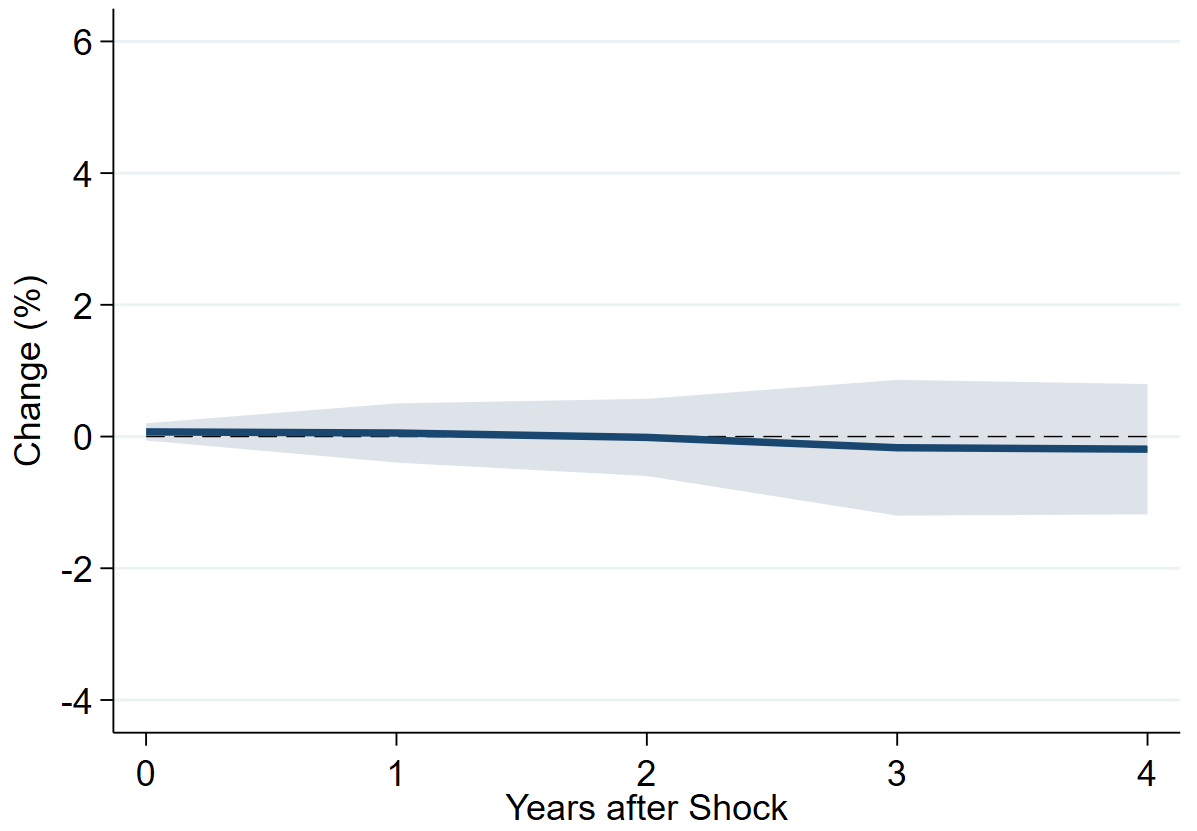
\includegraphics[height=1.5in,width=2.8in]{figures/graph_Rn_consexp_lv_Rn_ms_lv.png}} & & {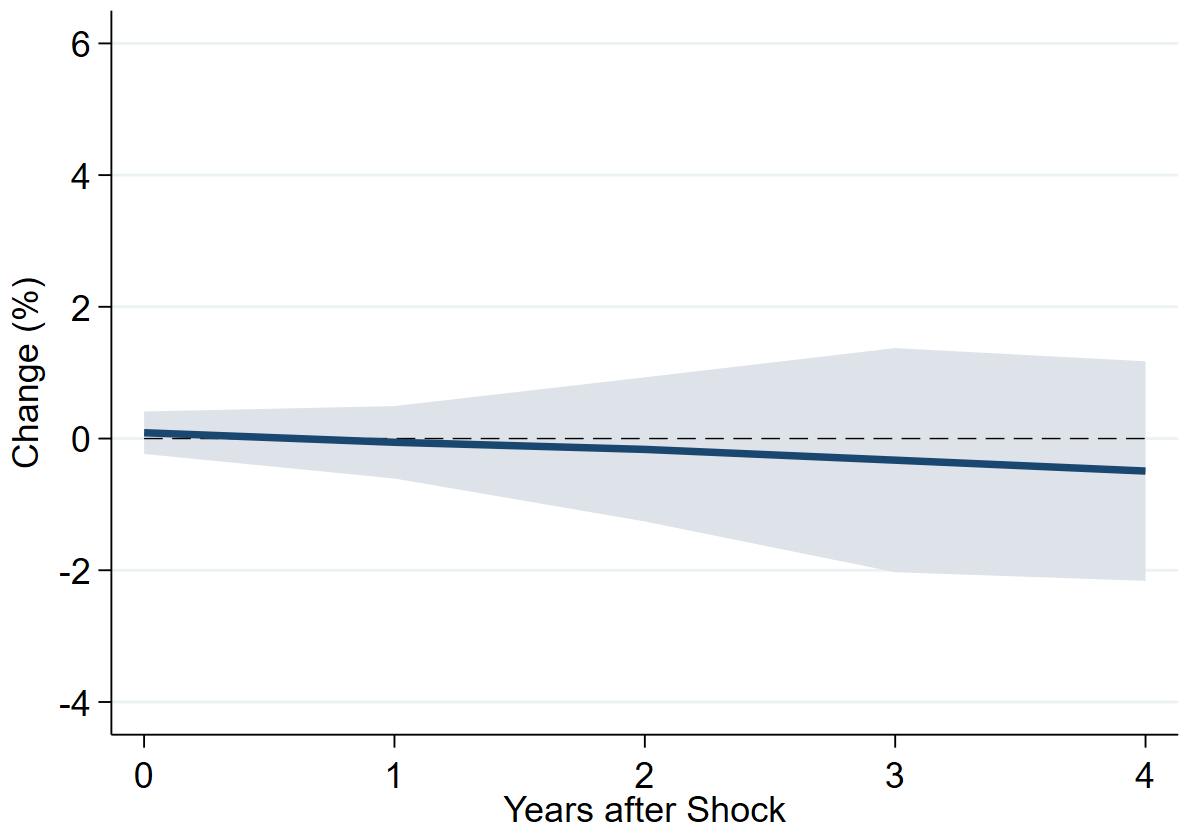
\includegraphics[height=1.5in,width=2.8in]{figures/graph_Rn_consexp_lv_Rn_ms_goods_lv.png}} \\[0.1in]
    
    \normalsize{\bf Panel C: Spending in Services} & & \normalsize{\bf Panel D: Spending in R\&D} \\
    {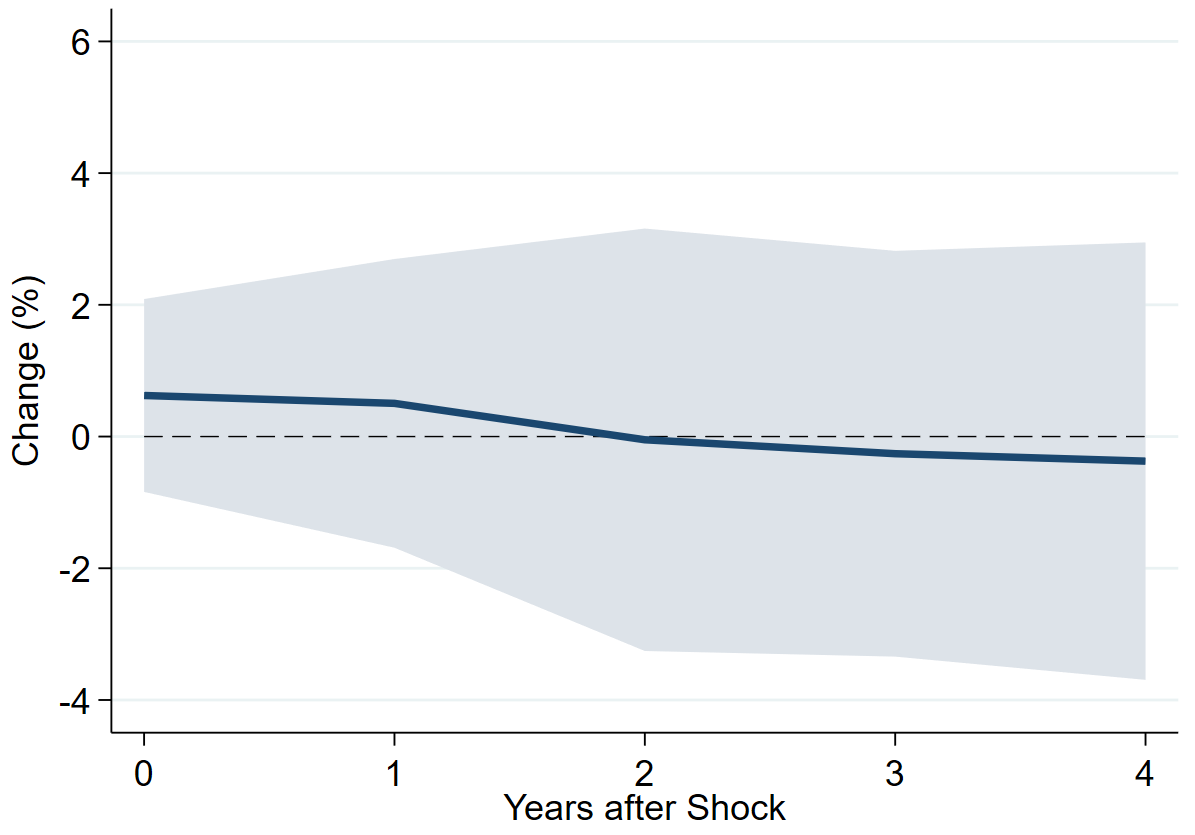
\includegraphics[height=1.5in,width=2.8in]{figures/graph_Rn_consexp_lv_Rn_ms_services_lv.png}} & & {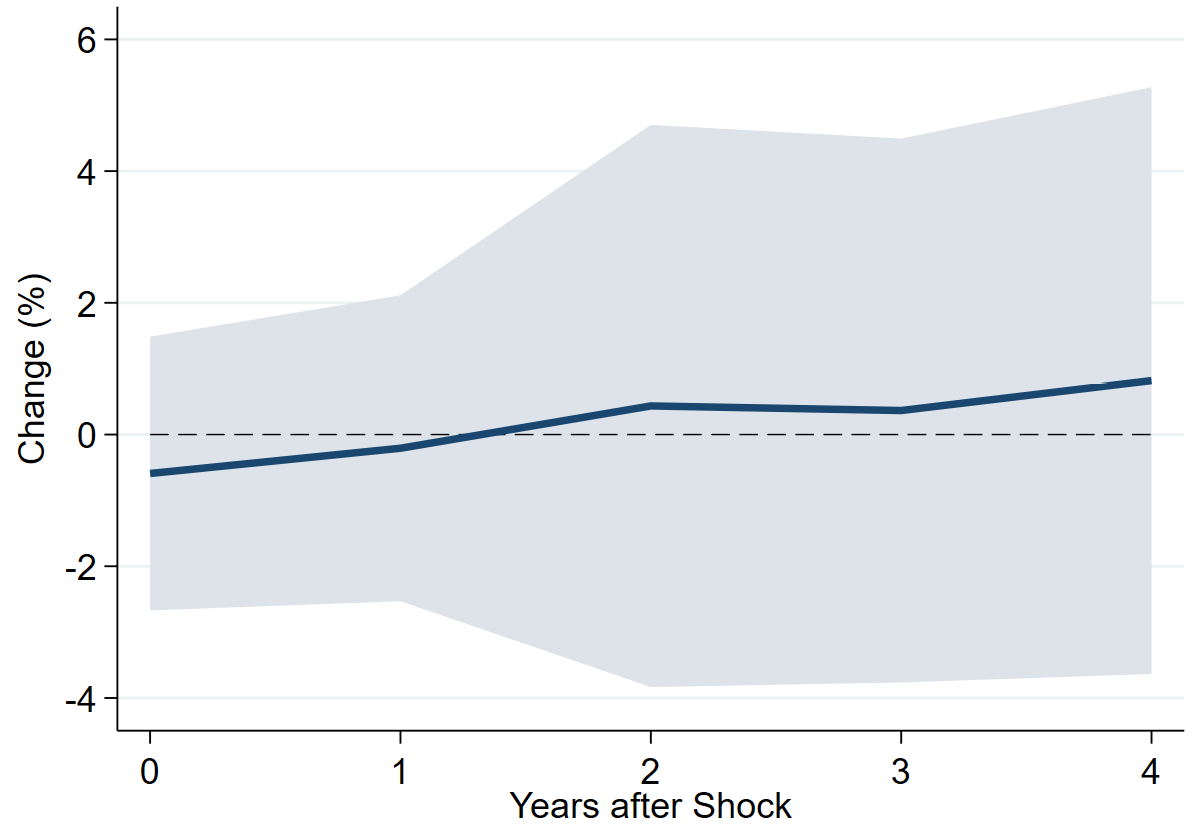
\includegraphics[height=1.5in,width=2.8in]{figures/graph_Rn_consexp_lv_Rn_ms_rd_lv.png}} \\[0.1in]

    
    \end{tabular}
    \caption{Private Consumption Crowding-out Effect}
    \end{center}
    
    
    
    
    \footnotesize{\textit{Note. } The unit of observations are states in different years. The balanced panel used for computing the estimates includes $51$ states for the period $1998-2015$. The instrument is calculated using observations between $1966$ and $1980$. Standard errors are clustered at state-level. The shaded areas report the $90\%$ confidence intervals.}

    \label{fig:crowd_privcons}
\end{figure}
\newpage


\newpage
\end{document}


\begin{comment}
   
\begin{figure}[ht]
    \begin{center}
        \begin{tabular}[c]{ccc}
    
    \normalsize{\bf Panel A: Total Spending} & & \normalsize{\bf Panel B: Spending in Goods} \\
    {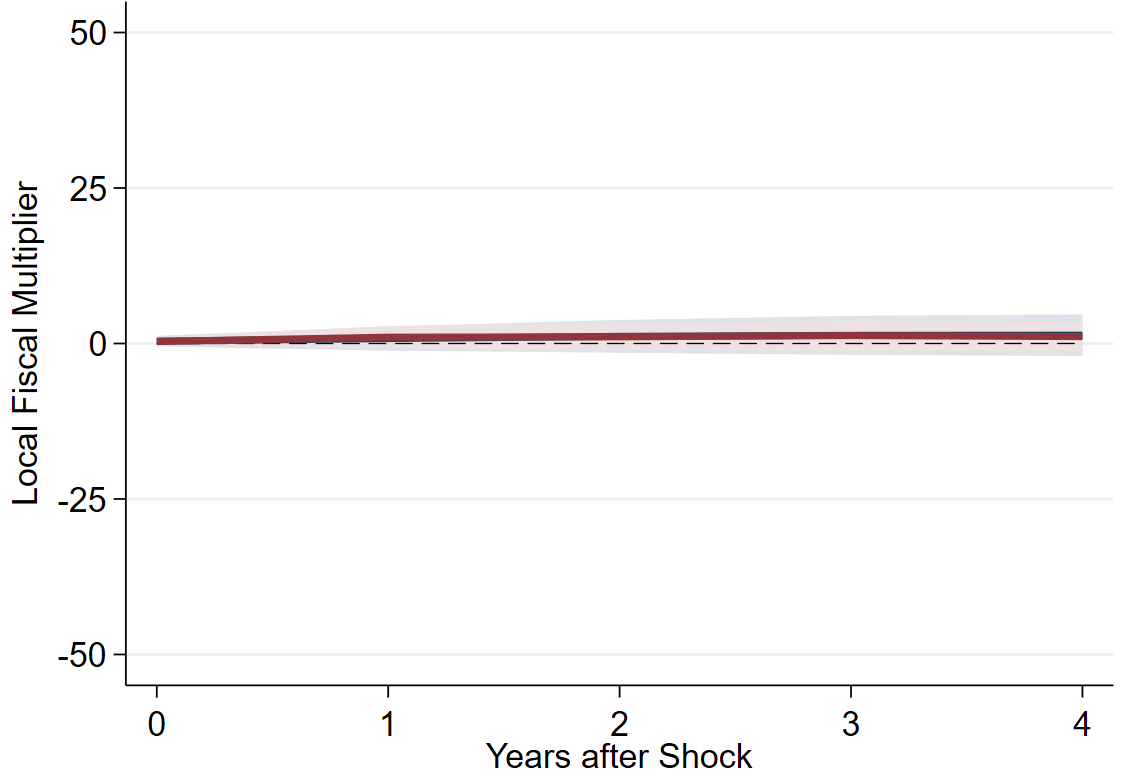
\includegraphics[height=1.5in,width=2.8in]{figures/graph_mpc_ms.png}} & & {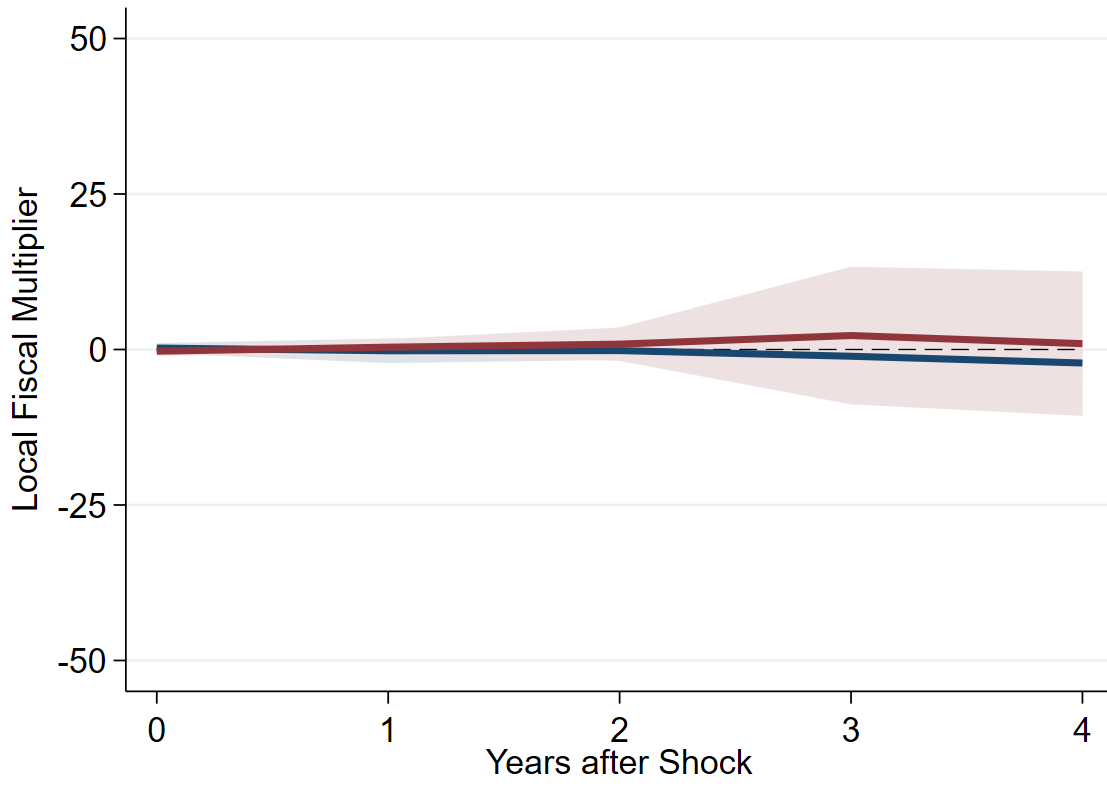
\includegraphics[height=1.5in,width=2.8in]{figures/graph_mpc_goods.png}} \\[0.1in]
    
    \normalsize{\bf Panel C: Spending in Services} & & \normalsize{\bf Panel D: Spending in R\&D} \\
    {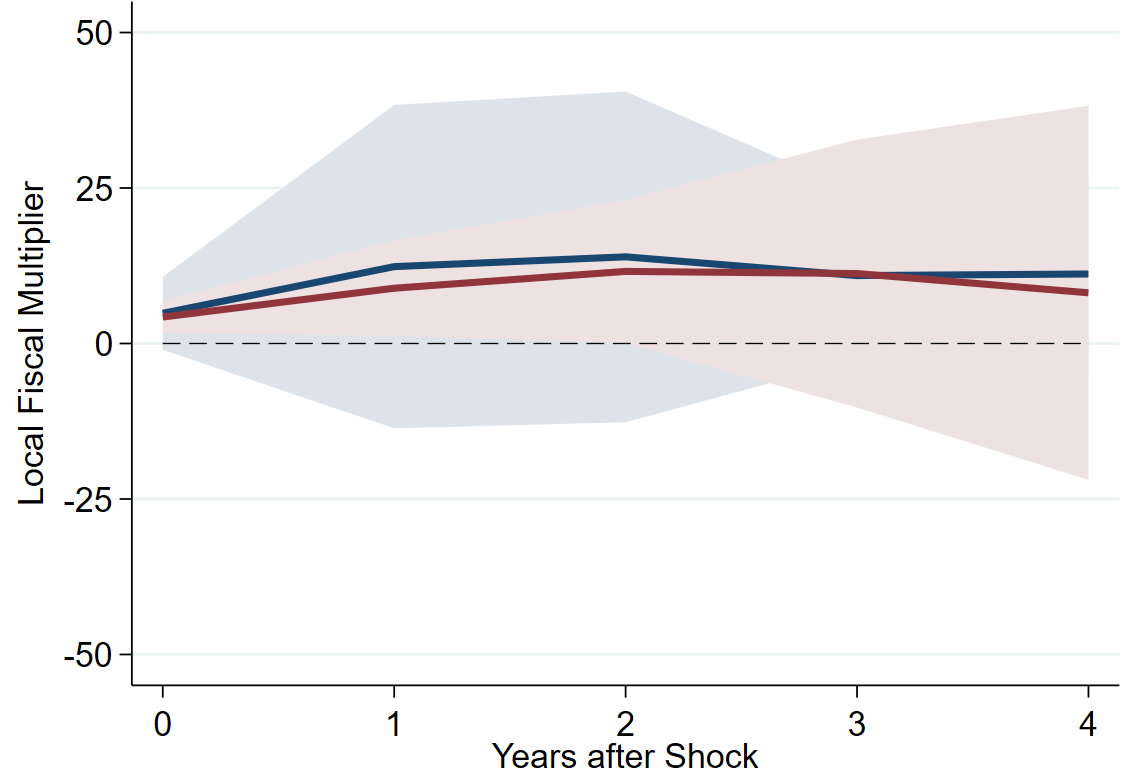
\includegraphics[height=1.5in,width=2.8in]{figures/graph_mpc_services.png}} & & {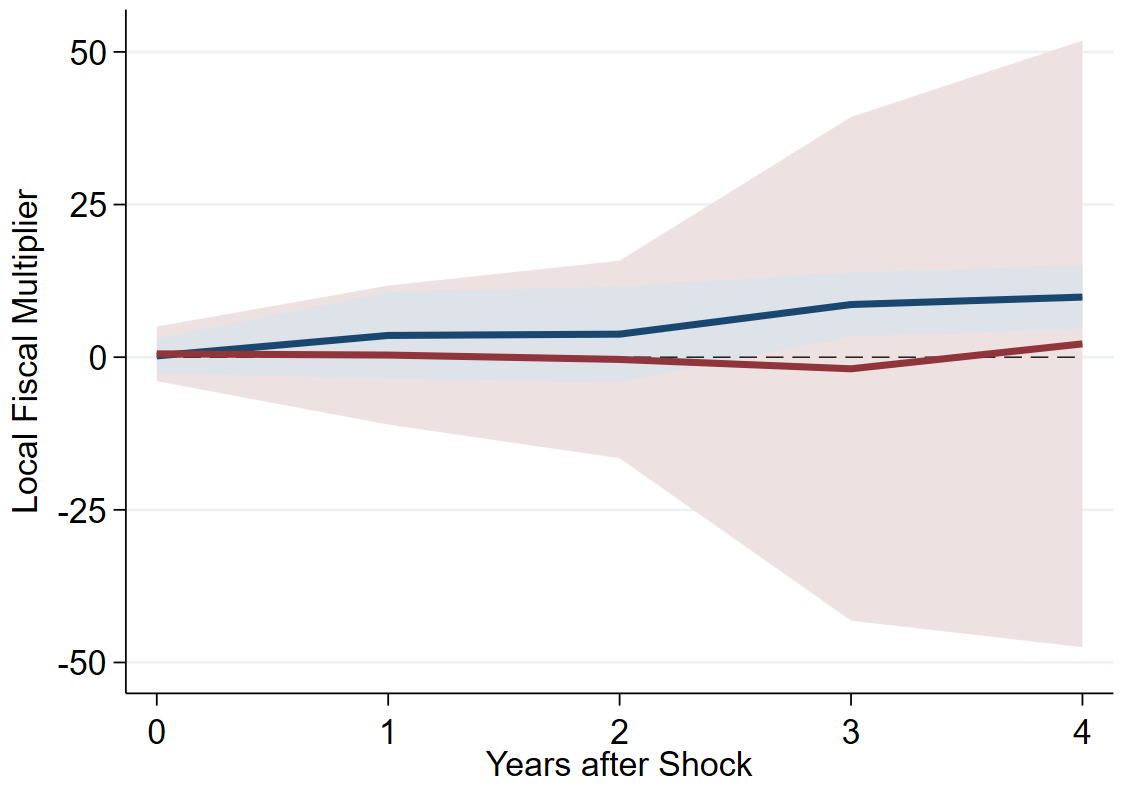
\includegraphics[height=1.5in,width=2.8in]{figures/graph_mpc_rd.png}} \\[0.1in]
    
    \multicolumn{3}{c}{
\includegraphics[height=0.15in,width=2.8in]{figures/graph_mpc_legend.png}} \\[0.1in]

    
    \end{tabular}
    \end{center}
    
    
    
    \caption{Fiscal Multiplier by High- vs. Low-MPC States}
    
    \footnotesize{\textit{Note. } The unit of observations are states in different years. The balanced panel used for computing the estimates includes $27$ states for the period $1980-2015$. The instrument is calculated using observations between $1966$ and $1980$. Standard errors are clustered at state-level. The shaded areas report the $90\%$ confidence intervals.}

    \label{fig:mpc}
\end{figure}
\end{comment}
    